\begin{frame}{The Closed-Set Assumption Behind a Classifier}
  \begin{columns}[T,onlytextwidth]
    \column{0.40\textwidth}
      \begin{itemize}\footnotesize\itemsep0.45em
        \item A benchmark such as ImageNet fixes three things before training starts:
        \begin{itemize}\scriptsize\itemsep0.15em
          \item a label set of $K$ classes;
          \item test images drawn from the same distribution as the training images;
          \item every test image belongs to one of the $K$ classes.
        \end{itemize}
        \item A softmax head (covered earlier) builds the first and the last into the model: it spreads a probability of 1 over the same $K$ labels for every input, including an image of something else.
        \item Deployed recognition breaks each assumption, and each break needs a different tool.
      \end{itemize}
    \column{0.58\textwidth}
      \centering
      \vspace{0.4em}
      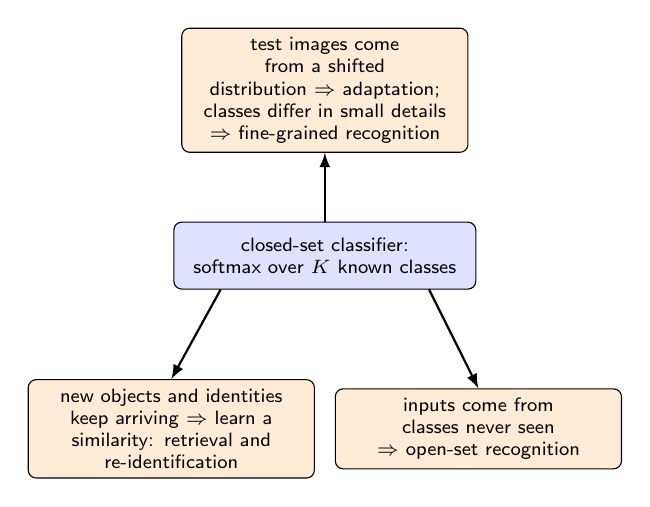
\begin{tikzpicture}[font=\sffamily\scriptsize, >=latex,
          box/.style={draw, rounded corners=0.1cm, align=center, minimum height=0.85cm},
          core/.style={box, fill=blue!12, text width=3.6cm},
          brk/.style={box, fill=orange!16, text width=3.4cm}]
        \node[core] (clf) at (0,0) {closed-set classifier:\\softmax over $K$ known classes};
        \node[brk] (fg) at (0,2.1) {test images come from a shifted\\distribution $\Rightarrow$ adaptation;\\classes differ in small details\\$\Rightarrow$ fine-grained recognition};
        \node[brk] (ml) at (-1.95,-2.2) {new objects and identities\\keep arriving $\Rightarrow$ learn a\\similarity: retrieval and\\re-identification};
        \node[brk] (os) at (1.95,-2.2) {inputs come from\\classes never seen\\$\Rightarrow$ open-set recognition};
        \draw[->, thick] (clf) -- (fg);
        \draw[->, thick] (clf.south west) ++(0.6,0) -- (ml.north);
        \draw[->, thick] (clf.south east) ++(-0.6,0) -- (os.north);
      \end{tikzpicture}\\[0.4em]
      {\scriptsize The three parts of this lecture, one per broken assumption; fine-grained recognition is the closed set at its hardest.\par}
  \end{columns}
\end{frame}

\begin{frame}{Recognition at Three Levels of Granularity}
  \centering
  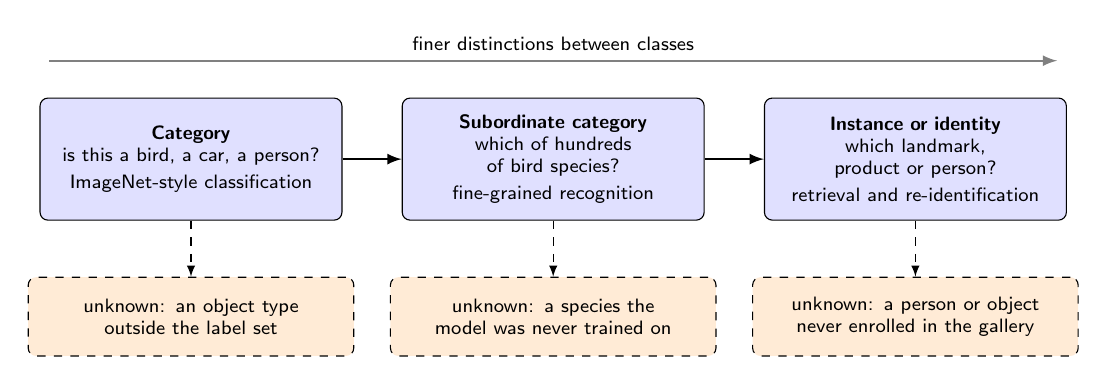
\begin{tikzpicture}[font=\sffamily\scriptsize, >=latex,
      lvl/.style={draw, rounded corners=0.1cm, align=center, fill=blue!12, text width=3.6cm, minimum height=1.55cm},
      unk/.style={draw, dashed, rounded corners=0.1cm, align=center, fill=orange!16, text width=3.9cm, minimum height=1.0cm}]
    \node[lvl] (cat) at (0,0) {\textbf{Category}\\is this a bird, a car, a person?\\[0.2em] ImageNet-style classification};
    \node[lvl] (sub) at (4.6,0) {\textbf{Subordinate category}\\which of hundreds of bird species?\\[0.2em] fine-grained recognition};
    \node[lvl] (ins) at (9.2,0) {\textbf{Instance or identity}\\which landmark, product or person?\\[0.2em] retrieval and re-identification};
    \draw[->, thick] (cat) -- (sub);
    \draw[->, thick] (sub) -- (ins);
    \node[unk] (u1) at (0,-2.0) {unknown: an object type\\outside the label set};
    \node[unk] (u2) at (4.6,-2.0) {unknown: a species the\\model was never trained on};
    \node[unk] (u3) at (9.2,-2.0) {unknown: a person or object\\never enrolled in the gallery};
    \draw[->, dashed] (cat) -- (u1);
    \draw[->, dashed] (sub) -- (u2);
    \draw[->, dashed] (ins) -- (u3);
    \draw[->, thick, gray] (-1.8,1.25) -- (11.0,1.25) node[midway, above, text=black] {finer distinctions between classes};
  \end{tikzpicture}\\[0.8em]
  \begin{itemize}\footnotesize\itemsep0.3em
    \item Moving right, classes become so numerous and so similar that a fixed softmax head stops being practical: at the instance level every object or person is its own class, and the system compares images instead of predicting a label.
    \item The dashed row is present at every level: whatever the granularity, some test inputs belong to no known class.
  \end{itemize}
\end{frame}

\begin{frame}{Three Questions a Recognition System Answers}
  \centering
  \vspace{0.3em}
  {\scriptsize
  \begin{tabular}{>{\raggedright\arraybackslash}p{3.3cm} >{\raggedright\arraybackslash}p{1.9cm} >{\raggedright\arraybackslash}p{3.3cm} >{\raggedright\arraybackslash}p{3.6cm}}
    \toprule
    \textbf{Question} & \textbf{Output} & \textbf{What is learned} & \textbf{How it is scored} \\
    \midrule
    Which of my $K$ classes is this, even when classes differ in small details? & one label & a classifier on adapted pretrained features & top-1 accuracy, in distribution and under distribution shift \\
    \addlinespace[0.35em]
    Which stored images show the same object, place or person? & a ranked list & an embedding whose distances reflect similarity or identity & how often a correct match appears among the top-ranked results; mean average precision \\
    \addlinespace[0.35em]
    Is this one of my classes at all? & a label or ``unknown'' & a classifier, a score of how known the input looks, and a rejection threshold & how well the score separates known from unknown inputs \\
    \bottomrule
  \end{tabular}\par}
  \vspace{0.8em}
  \begin{itemize}\footnotesize\itemsep0.35em
    \item The rows follow the lecture: classification and fine-grained recognition; metric learning, retrieval and re-identification; open-set recognition.
    \item Pretrained encoders such as CLIP and DINOv2 (covered earlier) changed all three rows. Each part asks what a frozen encoder already provides and what still has to be trained.
  \end{itemize}
\end{frame}
